\documentclass[final]{beamer}
\usepackage{outlines}
\usepackage{graphicx}
\usepackage{float}
\usepackage{mhchem}
\usepackage{amsmath}
\usepackage{amssymb}
\usepackage[T1]{fontenc}
\usepackage{tikz}
\usepackage{lmodern}
\usepackage{geometry}
\usepackage{caption}
\usepackage{wrapfig}
\usepackage{qrcode}
%\usepackage{chemfig}
% max size is 48x36 inches. We want a 1.61:1 ratio
\usepackage[scale=1.0,size=custom,width=121.92, height=91.44, margins=2.54]{beamerposter}
%\usepackage{mol2chemfig}
\usetheme{gemini}
\usecolortheme{ndsu}
\newlength{\sepwidth}
\newlength{\colwidth}
\setlength{\sepwidth}{0.025\paperwidth}
\setlength{\colwidth}{0.3\paperwidth}
\newcommand{\separatorcolumn}{\begin{column}{\sepwidth}\end{column}}

\tikzstyle{block} = [draw, fill=white, rectangle,
    minimum height=3em, minimum width=6em]


\DeclareCaptionType{equ}[][]

\usepackage[backend=bibtex,style=chem-acs]{biblatex}
\addbibresource{poster_2023.bib}

\title{\huge qsarify: High performance machine learning software package for QSAR model development.}
\author{Stephen Szwiec \and Bakhtiyor Rasulev}
\institute[shortinst]{Department of Coatings and Polymeric Materials, North Dakota State University, Fargo, ND}
\addtobeamertemplate{headline}{}
{
	\begin{tikzpicture}[remember picture,overlay]
		\node [anchor=south east, inner sep=3cm] at ([xshift=0.0cm,yshift=81.0cm]current page.south east){\includegraphics[height=4cm]{NDSU.pdf}};
		%\node [anchor=south east, inner sep=3cm] at ([xshift=-60.0cm,yshift=1.0cm]current page.south east){\includegraphics[height=4cm]{qsarify_logo.png}};
	\end{tikzpicture}
}

\footercontent{
  \href{https://rasulev.org}{https://rasulev.org} \hfill
  Conference on Computational Science 2023 -- North Dakota State University, Fargo ND \hfill
  \href{https://stephenszwiec.github.io/qsarify/}{https://stephenszwiec.github.io/qsarify/}}
\begin{document}

	\begin{frame}[t]
		\begin{columns}[t]
			\begin{column}{\colwidth}
				\begin{block}{Abstract}
qsarify is a new software package for the development, validation, and visualization of machine learning models for Quantitative Structure-Activity Relationship (QSAR) and Quantitative Structure-Property Relationship (QSPR) studies. Written in Python and freely available under the GNU General Public License, this software package provides a focused workflow for the generation of predictive statistical models to better explain and predict the relationship between molecular structure and biological activities or chemical properties. qsarify implements an innovative algorithm to reduce input dimensionality during the feature selection process, utilizing cophenetic clustering followed by a genetic algorithm (GA) for variable selection. Implementing both serial and parallel processing, this algorithm allows for rapid predictive model development and validation of large chemical datasets on low performance computers, while also allowing for complex model development and validation on high performance computers by utilizing multi-processing. Finally, the software also provides for output the of statistical validation metrics and generates plots for model diagnostics, including Williams Plot and Y-scrambling tests.
				\end{block}

				\begin{block}{Background}
					\large{\bfseries{QSAR and QSPR}} \smallskip

					\begin{itemize}
						\item QSAR and QSPR models are used to predict the biological activity or chemical properties of a compound based on its molecular structure, respectively.
						\item As a data driven approach, QSAR and QSPR models are developed using a combination of molecular descriptors and machine learning (ML) statistical regression models.
						\item QSAR and QSPR modeling is a powerful tool for the prediction of activity and properties of compounds, and allows for high throughput screening to be performed.
						\item QSAR and QSPR models are used in a variety of fields, including drug discovery, environmental chemistry, and materials science.
					\end{itemize}

					\large{\bfseries{Challenges}} \smallskip

					\begin{itemize}
						\item The development of QSAR and QSPR models is a time consuming process.
						\item Chemical descriptor calculation results in a large number of variables, which can be computationally intensive to process.
						\item Researcher hardware is often limited, and the development of QSAR and QSPR models can be computationally intensive.
						\item Current software packages are often proprietary, and are not freely available.
					\end{itemize}

					\large{\bfseries{Objectives}} \smallskip

					\begin{itemize}
						\item Develop a Free and Open Source Software (FOSS) package for the development, validation, and visualization of QSAR and QSPR models.
						\item Scale to the hardware available
						\item Automate workflows
						\item Rapidly develop and validate models
						\item Visualize relationships in data
					\end{itemize}

				\end{block}

				\begin{block}{Methods}

\large{\bfseries{Dimensionality Reduction}} \smallskip

					\begin{itemize}
						\item After processing the data, qsarify performs cophenetic clustering on descriptors \cite{rohlf1968}, reducing data dimensionality.
					\end{itemize}

					\begin{equ}{Cophenetic Clustering}
						\begin{equation}
							c = \frac{\sum_{i<j}^{n}[ d(i,j) - \bar{d}]}{[\sum_{i<j} d(i,j)]^2} \quad \text{where} \quad d(i,j) = \frac{\text{cov}(\vec{x}_i, \vec{x}_j)}{\sigma_i \sigma_j }
						\end{equation}
						\caption{Cophenetic correlation of the clustering based on the Euclidean distance $d$ of the Pearson correlation of each descriptor, creating hierarchical clustering.}
					\end{equ}

				\end{block}
			\end{column}

			\begin{column}{\colwidth}
				\begin{block}{Methods}
					\begin{columns}[t]
						\begin{column}{0.5\colwidth}


					\large{\bfseries{Genetic Algorithm}} \smallskip
					\begin{itemize}
						\item In the second step, a genetic algorithm (GA) is used to select the most important variables from the clustered descriptors.
						\item Progressively, the bank of models is refined until the $R^2$ score is maximized.
						\item The system can be configured to use either single or multi-processing, using reflection.
						\item The GA is implemented using a map-filter-reduce paradigm, allowing for the parallelization of the GA.
					\end{itemize}
\large{\bfseries{Model validation}} \smallskip
					\begin{itemize}
						\item The model is validated using the test set, and the $R^2$, $Q^2$, and $RMSE$ scores are calculated.
						\item The model is also validated using the Williams Plot and Y-scrambling tests.
						\item The model can also be further validated using a leave-one-out cross validation (LOOCV) test, and allows for additional QSAR-specific metrics ($Q^2_{f3}$ and $CCC$) to be provided.
					\end{itemize}

					\end{column}
					\begin{column}{0.5\colwidth}
						\begin{figure}
							\centering
							\includegraphics[width=0.5\colwidth]{process}
							\caption{diagram of qsarify workflow}
						\end{figure}

					\end{column}
				\end{columns}
						\begin{figure}
						\centering
						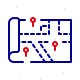
\includegraphics[width=0.4\colwidth]{map}
						\caption{map function applies the evolutionary algorithm to a bank of models}
						\end{figure}
			\end{block}
			\begin{block}{Testing}
				\begin{columns}[t]
					\begin{column}{\colwidth}
						\large{\bfseries{Nitro-aromatic Toxicity Prediction}} \smallskip
						\begin{itemize}
							\item The software was tested using a set of 28 nitro-aromatic compounds taken from literature \cite{rasulev2006}.
							\item $X$: 676 descriptors were calculated using the \texttt{Dragon 6} software \cite{dragon6}.
							\item $Y$: published $\text{log}_{10}$ of the $\text{LD}_{50}$ values for each compound.
							\item The qsarify model was trained using a set of 22 compounds, and tested using a set of 6 compounds.
						\end{itemize}
						\large{\bfseries{Computational Benchmarking}} \smallskip
						\begin{itemize}
							\item During model training, the software was benchmarked for speed and memory usage on:
							\begin{itemize}
								\item HP EliteDesk 800 G5 SFF Mini Desktop PC
								\item Intel Core i7-9700 @ 3.0 GHz
								\item 16 GB RAM
								\item Linux 6.0.12-artix1-1 x86\_64
								\item Python 3.10.9 (main, Dec 25 2022) [GCC 11.1.0]
							\end{itemize}
						\end{itemize}
						\end{column}
					\end{columns}
				\end{block}
			\begin{block}{Results}


				\begin{table}[h]
					\centering
					\begin{tabular}{|c  | c |}
						\hline
						\large \textbf{Model} & \textbf{Y} = -1.453 * \textbf{RDF070v} - 96.40 * \textbf{X5Av} - 0.076 \\
						\hline
						\large \textbf{R$^{2}$} & 0.793 \\
						\hline
						\large \textbf{Q$^{2}$} & 0.710 \\
						\hline
						\large \textbf{RMSE} & 0.251 \\
						\hline
					\end{tabular}
					\caption{Model performance statistics for an example two variable model.}
				\end{table}
			\end{block}

			\end{column}

			\begin{column}{\colwidth}

					\begin{block}{Results}

					\begin{columns}[t]
					\begin{column}{0.5\colwidth}
				\begin{figure}
					\centering
					
\includegraphics[width=0.45\colwidth]{cl.png}
					\caption{Histogram of autocorrelation coefficients of the clustering.}
				\end{figure}

				\begin{figure}
					\centering
					\includegraphics[width=0.45\colwidth]{te.png}
					\caption{predicted vs actual values for training and testing.}
				\end{figure}
				\end{column}
				\begin{column}{0.5\colwidth}
				\begin{figure}
					\centering
					\includegraphics[width=0.45\colwidth]{wi.png}
					\caption{Williams plot for training and testing; figure shows the leverage and residuals of the model, giving an applicability domain.}
				\end{figure}

				\begin{figure}
					\centering
					\includegraphics[width=0.45\colwidth]{ys.png}
					\caption{Y-scrambled plot for training and testing.}
				\end{figure}
				\end{column}
				\end{columns}

				\large{\bfseries{Computational Benchmarking}} \smallskip
				\begin{itemize}
					\item \textbf{Single core performance:} 0.20 seconds per learning cycle
					\item \textbf{Multi-core performance:} 0.089 seconds per learning cycle
					\item \textbf{Profiled memory usage:} 4.2 GiB per learning cycle
				\end{itemize}

				\end{block}

				\begin{block}{Conclusions}

				% Describe the conclusions of the project
				% Describe the significance of the project
				% Describe the significance of the results
				% Describe the significance of the future work

				\begin{itemize}
					\item \large Modern machine learning techniques can be delivered in a simple, easy to use package.
					\item \large Low performance computers can be used to train models with high predictive power in a short amount of time by combining dimensional reduction with smart algorithms.
					\item \large Software freedom is important for the future of science, and the qsarify library is a step in that direction for computational chemistry.
				\end{itemize}
				\end{block}
				\begin{column}{0.475\colwidth}
				\begin{block}{Current Release}
				\large{The current release of qsarify is available on PyPI and GitHub.}
				\begin{figure}
					\centering
					\qrcode[height=0.5\textwidth]{https://stephenszwiec.github.io/qsarify/}
				\end{figure}
				\end{block}
				\end{column}
				\begin{column}{0.475\colwidth}
				\begin{block}{ Acknowledgments}
				 Authors acknowledge the support from the National Science Foundation under grant number NSF CHE-1800476. In this work the super-computing resources of the Center for Computationally Assisted Science and Technology (CCAST) at North Dakota State University were used, which was made possible in part by NSF MRI Award No. 2019077 and by the State of North Dakota.
				\end{block}
			\end{column}
				\begin{block}{References}
					\printbibliography
				\end{block}
			\end{column}
		\end{columns}
	\end{frame}
\end{document}
